% Options for packages loaded elsewhere
\PassOptionsToPackage{unicode}{hyperref}
\PassOptionsToPackage{hyphens}{url}
\PassOptionsToPackage{dvipsnames,svgnames,x11names}{xcolor}
%
\documentclass[
  letterpaper,
  DIV=11,
  numbers=noendperiod]{scrartcl}

\usepackage{amsmath,amssymb}
\usepackage{iftex}
\ifPDFTeX
  \usepackage[T1]{fontenc}
  \usepackage[utf8]{inputenc}
  \usepackage{textcomp} % provide euro and other symbols
\else % if luatex or xetex
  \usepackage{unicode-math}
  \defaultfontfeatures{Scale=MatchLowercase}
  \defaultfontfeatures[\rmfamily]{Ligatures=TeX,Scale=1}
\fi
\usepackage{lmodern}
\ifPDFTeX\else  
    % xetex/luatex font selection
\fi
% Use upquote if available, for straight quotes in verbatim environments
\IfFileExists{upquote.sty}{\usepackage{upquote}}{}
\IfFileExists{microtype.sty}{% use microtype if available
  \usepackage[]{microtype}
  \UseMicrotypeSet[protrusion]{basicmath} % disable protrusion for tt fonts
}{}
\makeatletter
\@ifundefined{KOMAClassName}{% if non-KOMA class
  \IfFileExists{parskip.sty}{%
    \usepackage{parskip}
  }{% else
    \setlength{\parindent}{0pt}
    \setlength{\parskip}{6pt plus 2pt minus 1pt}}
}{% if KOMA class
  \KOMAoptions{parskip=half}}
\makeatother
\usepackage{xcolor}
\setlength{\emergencystretch}{3em} % prevent overfull lines
\setcounter{secnumdepth}{-\maxdimen} % remove section numbering
% Make \paragraph and \subparagraph free-standing
\makeatletter
\ifx\paragraph\undefined\else
  \let\oldparagraph\paragraph
  \renewcommand{\paragraph}{
    \@ifstar
      \xxxParagraphStar
      \xxxParagraphNoStar
  }
  \newcommand{\xxxParagraphStar}[1]{\oldparagraph*{#1}\mbox{}}
  \newcommand{\xxxParagraphNoStar}[1]{\oldparagraph{#1}\mbox{}}
\fi
\ifx\subparagraph\undefined\else
  \let\oldsubparagraph\subparagraph
  \renewcommand{\subparagraph}{
    \@ifstar
      \xxxSubParagraphStar
      \xxxSubParagraphNoStar
  }
  \newcommand{\xxxSubParagraphStar}[1]{\oldsubparagraph*{#1}\mbox{}}
  \newcommand{\xxxSubParagraphNoStar}[1]{\oldsubparagraph{#1}\mbox{}}
\fi
\makeatother


\providecommand{\tightlist}{%
  \setlength{\itemsep}{0pt}\setlength{\parskip}{0pt}}\usepackage{longtable,booktabs,array}
\usepackage{calc} % for calculating minipage widths
% Correct order of tables after \paragraph or \subparagraph
\usepackage{etoolbox}
\makeatletter
\patchcmd\longtable{\par}{\if@noskipsec\mbox{}\fi\par}{}{}
\makeatother
% Allow footnotes in longtable head/foot
\IfFileExists{footnotehyper.sty}{\usepackage{footnotehyper}}{\usepackage{footnote}}
\makesavenoteenv{longtable}
\usepackage{graphicx}
\makeatletter
\newsavebox\pandoc@box
\newcommand*\pandocbounded[1]{% scales image to fit in text height/width
  \sbox\pandoc@box{#1}%
  \Gscale@div\@tempa{\textheight}{\dimexpr\ht\pandoc@box+\dp\pandoc@box\relax}%
  \Gscale@div\@tempb{\linewidth}{\wd\pandoc@box}%
  \ifdim\@tempb\p@<\@tempa\p@\let\@tempa\@tempb\fi% select the smaller of both
  \ifdim\@tempa\p@<\p@\scalebox{\@tempa}{\usebox\pandoc@box}%
  \else\usebox{\pandoc@box}%
  \fi%
}
% Set default figure placement to htbp
\def\fps@figure{htbp}
\makeatother

\KOMAoption{captions}{tableheading}
\makeatletter
\@ifpackageloaded{caption}{}{\usepackage{caption}}
\AtBeginDocument{%
\ifdefined\contentsname
  \renewcommand*\contentsname{Table of contents}
\else
  \newcommand\contentsname{Table of contents}
\fi
\ifdefined\listfigurename
  \renewcommand*\listfigurename{List of Figures}
\else
  \newcommand\listfigurename{List of Figures}
\fi
\ifdefined\listtablename
  \renewcommand*\listtablename{List of Tables}
\else
  \newcommand\listtablename{List of Tables}
\fi
\ifdefined\figurename
  \renewcommand*\figurename{Figure}
\else
  \newcommand\figurename{Figure}
\fi
\ifdefined\tablename
  \renewcommand*\tablename{Table}
\else
  \newcommand\tablename{Table}
\fi
}
\@ifpackageloaded{float}{}{\usepackage{float}}
\floatstyle{ruled}
\@ifundefined{c@chapter}{\newfloat{codelisting}{h}{lop}}{\newfloat{codelisting}{h}{lop}[chapter]}
\floatname{codelisting}{Listing}
\newcommand*\listoflistings{\listof{codelisting}{List of Listings}}
\makeatother
\makeatletter
\makeatother
\makeatletter
\@ifpackageloaded{caption}{}{\usepackage{caption}}
\@ifpackageloaded{subcaption}{}{\usepackage{subcaption}}
\makeatother

\usepackage{bookmark}

\IfFileExists{xurl.sty}{\usepackage{xurl}}{} % add URL line breaks if available
\urlstyle{same} % disable monospaced font for URLs
\hypersetup{
  pdftitle={CompanionBot},
  colorlinks=true,
  linkcolor={blue},
  filecolor={Maroon},
  citecolor={Blue},
  urlcolor={Blue},
  pdfcreator={LaTeX via pandoc}}


\title{CompanionBot}
\usepackage{etoolbox}
\makeatletter
\providecommand{\subtitle}[1]{% add subtitle to \maketitle
  \apptocmd{\@title}{\par {\large #1 \par}}{}{}
}
\makeatother
\subtitle{Final Project for the Adavance Software Development Methods
Course}
\author{Andrey Malyukov \and Anton Voronov \and Nikita
Podstrelov \and Aleksandr Grinbaum \and Solomon Naftaliyev \and Bohdan
Zachepa \and Nikita Popilin}
\date{2025-06-24}

\begin{document}
\maketitle

\renewcommand*\contentsname{Table of contents}
{
\hypersetup{linkcolor=}
\setcounter{tocdepth}{3}
\tableofcontents
}

\begin{figure}[H]

{\centering \pandocbounded{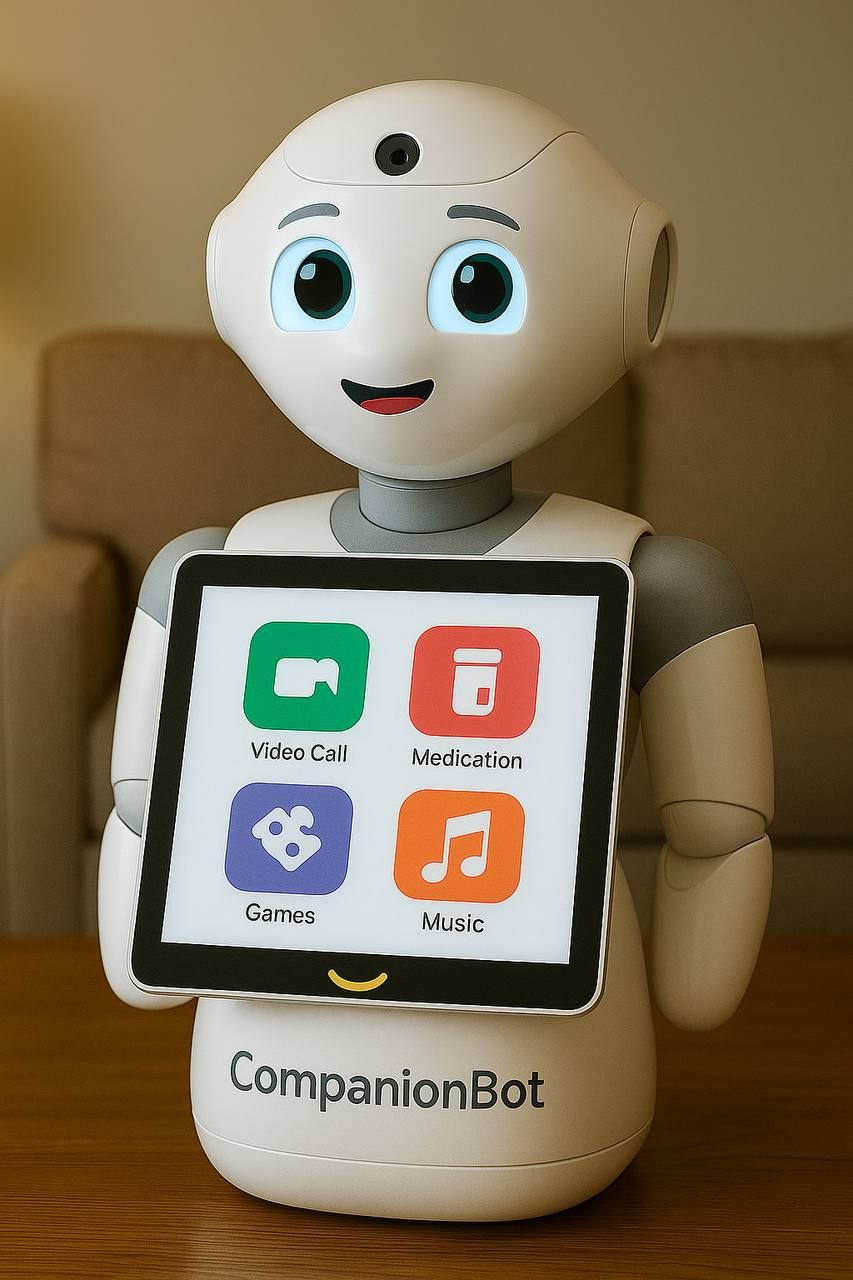
\includegraphics[keepaspectratio]{./images/robot-image.jpg}}

}

\caption{Artistic Representation of CompanionBot}

\end{figure}%

\section{1. CompanionBot: System Definition and
Super-Characterization}\label{companionbot-system-definition-and-super-characterization}

\subsection{Purpose of the System}\label{purpose-of-the-system}

CompanionBot is an AI-driven digital companion designed to enhance the
quality of life for seniors by addressing several critical challenges in
elderly care:

\begin{itemize}
\tightlist
\item
  \textbf{Social Isolation and Loneliness:} Providing consistent
  companionship and facilitating connections with family, friends, and
  peer communities.
\item
  \textbf{Health Management Complexity:} Offering structured assistance
  with medication adherence, health monitoring, and wellness activities.
\item
  \textbf{Cognitive Engagement:} Delivering personalized mental
  stimulation to maintain cognitive function and prevent decline.
\item
  \textbf{Technology Bridge:} Serving as an accessible gateway between
  seniors, their families, and modern digital technologies.
\end{itemize}

The system aims to complement, not replace, human care by providing 24/7
availability, consistent interaction quality, and personalized support
tailored to individual user needs and preferences.

\subsection{What the System Will Do}\label{what-the-system-will-do}

\subsubsection{Core Functionalities}\label{core-functionalities}

\paragraph{Social Connection Module}\label{social-connection-module}

\begin{itemize}
\tightlist
\item
  Facilitate video calls with family members and friends through
  simplified interfaces.
\item
  Enable photo sharing and digital album creation for memory
  preservation.
\item
  Coordinate group activities with other CompanionBot users (virtual
  bingo, book clubs, discussion groups).
\item
  Provide daily conversational engagement with natural language
  processing and through a Large Language Model (LLM) capable of
  understanding user context and emotional tone.
\end{itemize}

\paragraph{Health Management Module}\label{health-management-module}

\begin{itemize}
\tightlist
\item
  Deliver personalized medication reminders with adherence tracking.
\item
  Guide users through age-appropriate exercise routines and physical
  activities.
\item
  Monitor vital signs through integrated health devices (blood pressure,
  pulse oximetry).
\item
  Facilitate meditation and relaxation sessions for mental wellness.
\item
  Track symptoms and maintain health journals for healthcare provider
  communication.
\item
  Provide hydration and nutrition reminders based on individual health
  needs.
\end{itemize}

\paragraph{Cognitive Engagement
Module}\label{cognitive-engagement-module}

\begin{itemize}
\tightlist
\item
  Offer adaptive brain games and puzzles tailored to user cognitive
  ability.
\item
  Engage in current events discussions and news updates.
\item
  Provide virtual travel experiences and cultural exploration.
\item
  Support music appreciation activities and personalized playlists.
\item
  Enable creative activities including poetry composition.
\end{itemize}

\paragraph{Smart Integration Module}\label{smart-integration-module}

\begin{itemize}
\tightlist
\item
  Control compatible smart home devices through voice commands.
\item
  Provide contextual awareness of home environment for safety
  monitoring.
\item
  Integrate with existing healthcare systems for seamless care
  coordination.
\item
  Support telehealth session facilitation and technical assistance.
\end{itemize}

\subsubsection{Advanced AI Capabilities}\label{advanced-ai-capabilities}

\begin{itemize}
\tightlist
\item
  \textbf{LLM-Powered Personalized Learning:} Integrates a Large
  Language Model to support flexible, natural, and emotionally aware
  dialogue. The LLM remembers user preferences, adapts interaction
  patterns, and provides personalized suggestions.
\item
  \textbf{Proactive Engagement:} Detects loneliness indicators and
  initiates appropriate interventions.
\item
  \textbf{Emotion Recognition:} Analyzes vocal patterns and facial
  expressions to provide empathetic responses.
\item
  \textbf{Context Awareness:} Understands user routines, preferences,
  and environmental factors for intelligent assistance.
\item
  \textbf{Multi-modal Interaction:} Supports voice, touch, gesture, and
  visual communication modalities.
\end{itemize}

\subsection{How Users Will Interact with the
System}\label{how-users-will-interact-with-the-system}

\subsubsection{Primary Interaction
Modalities}\label{primary-interaction-modalities}

\paragraph{Voice Interaction}\label{voice-interaction}

\begin{itemize}
\tightlist
\item
  Natural language conversation capabilities powered by an LLM, enabling
  contextual memory, multilingual support, and emotionally adaptive
  interaction.
\item
  Voice commands for system control and activity initiation.
\item
  Adjustable speech rate and volume for hearing accessibility.
\item
  Multi-language support for diverse user populations.
\end{itemize}

\paragraph{Touch Interface}\label{touch-interface}

\begin{itemize}
\tightlist
\item
  Large, high-contrast buttons on detachable tablet display.
\item
  Simplified navigation with minimal cognitive load.
\item
  Haptic feedback for confirmation of actions.
\item
  Customizable interface layouts based on user abilities.
\end{itemize}

\paragraph{Visual Interaction}\label{visual-interaction}

\begin{itemize}
\tightlist
\item
  Expressive robotic head with emotional LED indicators.
\item
  Video calling capabilities through integrated camera systems.
\item
  Photo sharing and viewing on high-resolution displays.
\item
  Gesture recognition for users with speech limitations.
\end{itemize}

\paragraph{Physical Interaction}\label{physical-interaction}

\begin{itemize}
\tightlist
\item
  Motion sensors for presence detection and automatic engagement.
\item
  Emergency alert pendant integration for safety monitoring.
\item
  Health device connectivity for seamless data collection.
\item
  Smart home device control through centralized hub.
\end{itemize}

\subsubsection{Accessibility Features}\label{accessibility-features}

The system accommodates a wide range of user needs:

\begin{itemize}
\tightlist
\item
  For visual impairments: high-contrast displays, large-text options,
  and voice guidance.
\item
  For hearing challenges: visual indicators, adjustable volume controls,
  and text-to-speech alternatives.
\item
  For motor difficulties: multiple input methods, simplified gestures,
  and voice-operated controls.
\item
  For cognitive assistance: consistent interfaces, clear instructions,
  and patient repetition.
\end{itemize}

\subsection{Who Will Use the System}\label{who-will-use-the-system}

\subsubsection{Primary Users}\label{primary-users}

\paragraph{Independent Seniors}\label{independent-seniors}

\begin{itemize}
\tightlist
\item
  Living independently in their own homes.
\item
  Experiencing mild to moderate social isolation.
\item
  Managing multiple medications and health conditions.
\item
  Seeking to maintain cognitive function and social connections.
\end{itemize}

\paragraph{Seniors with Mild Cognitive
Decline}\label{seniors-with-mild-cognitive-decline}

\begin{itemize}
\tightlist
\item
  Early-stage dementia or mild cognitive impairment.
\item
  Requiring structured daily routines and medication reminders.
\item
  Benefiting from consistent social interaction and mental stimulation.
\item
  Need for simplified, patient technology interfaces.
\end{itemize}

\paragraph{Socially Isolated Seniors}\label{socially-isolated-seniors}

\begin{itemize}
\tightlist
\item
  Limited family contact or geographic separation from loved ones.
\item
  Reduced mobility affecting social activities.
\item
  Recent life transitions (widowhood, retirement, relocation).
\item
  Seeking meaningful social connections and daily structure.
\end{itemize}

\subsubsection{Secondary Users}\label{secondary-users}

\paragraph{Family Members and
Caregivers}\label{family-members-and-caregivers}

\begin{itemize}
\tightlist
\item
  Adult children monitoring elderly parents' wellbeing.
\item
  Professional caregivers coordinating care plans.
\item
  Healthcare providers accessing health data and communication.
\item
  Social workers and community health coordinators.
\end{itemize}

\paragraph{Healthcare Professionals}\label{healthcare-professionals}

\begin{itemize}
\tightlist
\item
  Primary care physicians monitoring patient adherence and health
  metrics.
\item
  Specialists requiring regular health data collection.
\item
  Mental health professionals tracking mood and cognitive function.
\item
  Pharmacists supporting medication management.
\end{itemize}

\subsection{Constraints (Privacy, Security,
Ethics)}\label{constraints-privacy-security-ethics}

\subsubsection{Privacy Constraints}\label{privacy-constraints}

\paragraph{Data Collection
Limitations}\label{data-collection-limitations}

\begin{itemize}
\tightlist
\item
  Explicit user consent required for all data collection activities.
\item
  Minimal data collection principle: only essential information
  gathered.
\item
  Local processing prioritized to reduce cloud data transmission.
\item
  Clear data retention policies with automatic deletion schedules.
\end{itemize}

\paragraph{Information Sharing
Controls}\label{information-sharing-controls}

\begin{itemize}
\tightlist
\item
  Granular permission settings for family access to health information.
\item
  Healthcare provider data sharing requires explicit medical consent.
\item
  Emergency protocol data sharing limited to life-threatening
  situations.
\item
  User ability to review and delete personal data at any time.
\end{itemize}

\subsubsection{Security Constraints}\label{security-constraints}

\paragraph{Technical Security
Requirements}\label{technical-security-requirements}

\begin{itemize}
\tightlist
\item
  End-to-end encryption for all data transmission.
\item
  Secure authentication protocols for family and caregiver access.
\item
  Regular security updates and vulnerability patching.
\item
  Physical device security features to prevent tampering.
\end{itemize}

\paragraph{Data Protection Standards}\label{data-protection-standards}

\begin{itemize}
\tightlist
\item
  HIPAA compliance for health-related information.
\item
  SOC 2 Type II certification for cloud infrastructure.
\item
  Regular third-party security audits and penetration testing.
\item
  Incident response procedures for data breaches.
\item
  Backup and disaster recovery protocols.
\end{itemize}

\subsubsection{Ethical Constraints}\label{ethical-constraints}

\paragraph{Autonomy and Dignity}\label{autonomy-and-dignity}

\begin{itemize}
\tightlist
\item
  Preservation of user independence and decision-making authority.
\item
  Transparent disclosure of AI capabilities and limitations.
\item
  Respect for cultural and religious preferences in care approaches.
\item
  User control over AI personality and interaction styles.
\end{itemize}

\paragraph{Deception and Authenticity}\label{deception-and-authenticity}

\begin{itemize}
\tightlist
\item
  Clear identification of AI vs.~human interactions.
\item
  Honest representation of AI emotional capabilities.
\item
  Avoidance of false promises regarding health outcomes.
\item
  Transparent explanation of data usage and AI decision-making.
\item
  Respect for user emotional investment in AI relationships.
\end{itemize}

\paragraph{Equity and Accessibility}\label{equity-and-accessibility}

\begin{itemize}
\tightlist
\item
  Affordable pricing models to prevent socioeconomic exclusion.
\item
  Support for users with various disability levels.
\item
  Multiple language support for diverse user populations.
\item
  Training and support resources for technology adoption.
\end{itemize}

\paragraph{Care Integration Ethics}\label{care-integration-ethics}

\begin{itemize}
\tightlist
\item
  Complement, not replace, human care relationships.
\item
  Support for maintaining family and social connections.
\item
  Integration with existing healthcare without disruption.
\item
  Respect for professional caregiver roles and expertise.
\item
  Transparency with healthcare providers about AI involvement.
\end{itemize}

\subsection{Scientific Reasoning and Research
Foundation}\label{scientific-reasoning-and-research-foundation}

\subsubsection{Loneliness and Social Isolation
Research}\label{loneliness-and-social-isolation-research}

The development of CompanionBot is grounded in extensive research
demonstrating the severe health impacts of loneliness in older adults.
Loneliness is a common problem in older adults and contributes to poor
health, with studies showing increased risks of depression, cognitive
decline, and mortality. Recent meta-analyses have demonstrated that
social robot interventions had significant positive effects on
decreasing depression and loneliness with large effect sizes.

Research specifically examining social robots for elderly care has shown
promising results. A comprehensive scoping review found that social
robots could tackle both emotional and social loneliness in assisted
living by empowering people to engage in different forms of social
interaction inside and outside the facility. Additionally, studies on
existing companion robots like ElliQ have provided valuable insights
into effective design principles and user acceptance patterns.

\textbf{Key Research Citations:}

\begin{itemize}
\tightlist
\item
  Norina Gasteiger et al.~(2021). ``Friends from the Future: A Scoping
  Review of Research into Robots and Computer Agents to Combat
  Loneliness in Older People.'' \emph{PMC}
\item
  Yen et al.~(2024). ``The Effect of Social Robots on Depression and
  Loneliness for Older Residents in Long-Term Care Facilities: A
  Meta-Analysis of Randomized Controlled Trials.'' \emph{PubMed}
\item
  Pirhonen et al.~(2020). ``Can robots tackle late-life loneliness?
  Scanning of future opportunities and challenges in assisted living
  facilities.'' \emph{ScienceDirect}
\end{itemize}

\subsubsection{Medication Management and Health
Compliance}\label{medication-management-and-health-compliance}

Research consistently demonstrates medication non-adherence as a
critical challenge in elderly care. Studies show that medication
non-adherence is a common problem with a high risk for severe
consequences, which can jeopardize older adults' health and
independence. Robotic interventions have shown significant promise, with
research indicating that using a robot for medication management had a
decreasing effect on home care professionals' use of working time while
improving health outcomes.

Clinical trials of robotic medication management systems have
demonstrated safety and usability, with all patients and 96\% of nurses
reporting the device was easy to use in pilot studies. Advanced
conversation-based systems using companion robots have been successfully
implemented and tested with positive user acceptance rates.

\textbf{Key Research Citations:}

\begin{itemize}
\tightlist
\item
  Prakash et al.~(2013). ``Older Adults' Medication Management in the
  Home: How can Robots Help?'' \emph{PMC}
\item
  Kajander-Unkuri et al.~(2023). ``Effect of robot for medication
  management on home care professionals' use of working time in older
  people's home care: a non-randomized controlled clinical trial.''
  \emph{PMC}
\item
  Su et al.~(2021). ``Conversation-Based Medication Management System
  for Older Adults Using a Companion Robot and Cloud.'' \emph{IEEE}
\end{itemize}

\subsubsection{Cognitive Engagement and Mental
Health}\label{cognitive-engagement-and-mental-health}

Research supports the importance of cognitive stimulation in maintaining
mental function among older adults. Studies examining companion robots
have found that companion robots should be accepted in the long-term by
older adults with mild cognitive decline in order to increase their use
and provide company, reduce loneliness, as well as to open the
possibility of using them for therapy via social interaction.

Recent research has emphasized the importance of personalized, adaptive
systems that can evolve with user needs. Older adults' expectations of
conversational companionship might substantially differ from what
current technologies can achieve, highlighting the need for advanced AI
systems with sophisticated natural language processing and emotional
intelligence capabilities.

\textbf{Key Research Citations:}

\begin{itemize}
\tightlist
\item
  Figueroa et al.~(2023). ``Social robot for older adults with cognitive
  decline: a preliminary trial.'' \emph{Frontiers in Robotics and AI}
\item
  Irfan et al.~(2024). ``Recommendations for designing conversational
  companion robots with older adults through foundation models.''
  \emph{Frontiers in Robotics and AI}
\item
  Tan et al.~(2024). ``Improving the Social Well-Being of Single Older
  Adults Using the LOVOT Social Robot: Qualitative Phenomenological
  Study'' \emph{JMIR Human Factors}
\end{itemize}

\section{2. Stakeholder Analysis and Decision-Making
Framework}\label{stakeholder-analysis-and-decision-making-framework}

\subsection{Primary Stakeholders}\label{primary-stakeholders}

\begin{longtable}[]{@{}
  >{\raggedright\arraybackslash}p{(\linewidth - 6\tabcolsep) * \real{0.0971}}
  >{\raggedright\arraybackslash}p{(\linewidth - 6\tabcolsep) * \real{0.2950}}
  >{\raggedright\arraybackslash}p{(\linewidth - 6\tabcolsep) * \real{0.2698}}
  >{\raggedright\arraybackslash}p{(\linewidth - 6\tabcolsep) * \real{0.3381}}@{}}
\toprule\noalign{}
\begin{minipage}[b]{\linewidth}\raggedright
Stakeholder
\end{minipage} & \begin{minipage}[b]{\linewidth}\raggedright
Primary Interests
\end{minipage} & \begin{minipage}[b]{\linewidth}\raggedright
Influence
\end{minipage} & \begin{minipage}[b]{\linewidth}\raggedright
Expectations
\end{minipage} \\
\midrule\noalign{}
\endhead
\bottomrule\noalign{}
\endlastfoot
Elderly Users & Ease of use, privacy, companionship, health monitoring,
dignity, social connection & High -- Direct users whose adoption and
satisfaction determine project success & Intuitive interface, reliable
functionality, respectful interaction, privacy protection \\
Family Members & Safety alerts, engagement updates, photo sharing,
crisis notifications, wellbeing & High -- Often primary decision-makers
for purchase and setup, ongoing support & Reliable alerts, easy
communication, health insights, low maintenance requirements \\
Healthcare Providers & Reliable medical alerts, actionable data, EHR
integration, reduced false positives & Medium-High -- May recommend or
discourage use based on perceived usefulness & Accurate health data,
integration with existing systems, evidence-based interventions \\
NGOs (AARP, WHO Ageing) & Accessibility, affordability, digital literacy
support, ethical AI use & Not specified & Not specified \\
Investors & Market scalability, ROI, regulatory compliance, user
adoption, revenue & High -- Control over budget, resources, strategic
direction & Viable product, clear market differentiation, positive
adoption metrics, ROI achievement \\
Regulators & HIPAA/GDPR/ADA compliance, safety certifications, data
sovereignty, ethical AI & Very High -- Can approve or block deployment
based on compliance assessment & Adherence to regulations, transparent
data practices, ethical AI implementation \\
Caregivers & Usability insights, behavioral trend reports, workload
reduction, wellbeing & High -- Often primary decision-makers for
purchase and setup, ongoing support & Reliable alerts, easy
communication, health insights, low maintenance requirements \\
Insurance providers & Risk mitigation, cost reduction, and preventive
care & Not specified & Not specified \\
Development Team & Creating effective, innovative solutions, technical
feasibility, professional growth & High -- Direct impact on product
capabilities, quality, and timeline & Clear requirements, realistic
timelines, necessary resources, technical autonomy \\
Technology Partners & Partnership success, technology integration,
market expansion & Medium -- Impact on technical capabilities and
integration success & Clear integration requirements, technical support,
revenue sharing agreements \\
\end{longtable}

\subsection{Decision-Making Framework}\label{decision-making-framework}

\subsubsection{Decision Authority
Matrix}\label{decision-authority-matrix}

\begin{longtable}[]{@{}
  >{\raggedright\arraybackslash}p{(\linewidth - 6\tabcolsep) * \real{0.2034}}
  >{\raggedright\arraybackslash}p{(\linewidth - 6\tabcolsep) * \real{0.2373}}
  >{\raggedright\arraybackslash}p{(\linewidth - 6\tabcolsep) * \real{0.2373}}
  >{\raggedright\arraybackslash}p{(\linewidth - 6\tabcolsep) * \real{0.3220}}@{}}
\toprule\noalign{}
\begin{minipage}[b]{\linewidth}\raggedright
Decision Type
\end{minipage} & \begin{minipage}[b]{\linewidth}\raggedright
Primary Decision Maker
\end{minipage} & \begin{minipage}[b]{\linewidth}\raggedright
Required Approvals
\end{minipage} & \begin{minipage}[b]{\linewidth}\raggedright
Consultation Required
\end{minipage} \\
\midrule\noalign{}
\endhead
\bottomrule\noalign{}
\endlastfoot
Strategic Direction & Business Stakeholders & Board/Investors & All
Primary Stakeholders \\
Product Features & Product Owner & Senior Users, Healthcare &
Development Team, Family Caregivers \\
Technical Architecture & Technical Lead & Business Stakeholders &
Development Team, Technology Partners \\
User Interface Design & UX Lead & Senior Users, NGOs, Family & Family,
Caregivers, NGOs \\
Health Features & Healthcare Advisory Board & Regulatory Bodies &
Healthcare Providers, Senior Users \\
Privacy/Security & Privacy Officer & Legal Team, Regulatory & All
Stakeholders \\
Budget Allocation & Financial Stakeholders & Business Leadership &
Project Management Team \\
Timeline/Milestones & Project Manager & Business Stakeholders &
Development Team, Key Stakeholders \\
Vendor Selection & Procurement Lead & Technical Lead, Financial &
Development Team \\
Go-to-Market Strategy & Marketing Lead & Business Stakeholders &
Healthcare Providers, Family, Caregivers \\
\end{longtable}

\subsubsection{Decision-Making Process}\label{decision-making-process}

\paragraph{Level 1: Operational Decisions (Daily
Development)}\label{level-1-operational-decisions-daily-development}

\begin{itemize}
\tightlist
\item
  \textbf{Authority:} Development Team Leads
\item
  \textbf{Process:} Agile methodology, daily standups, sprint planning
\item
  \textbf{Timeline:} Immediate to 2 weeks
\item
  \textbf{Documentation:} Sprint logs, technical documentation
\item
  \textbf{Review:} Weekly team retrospectives
\end{itemize}

\paragraph{Level 2: Tactical Decisions (Feature and
Design)}\label{level-2-tactical-decisions-feature-and-design}

\begin{itemize}
\tightlist
\item
  \textbf{Authority:} Product Owner with Stakeholder Input
\item
  \textbf{Process:}

  \begin{enumerate}
  \def\labelenumi{\arabic{enumi}.}
  \tightlist
  \item
    Stakeholder consultation (1 week)
  \item
    Impact analysis (3-5 days)
  \item
    Decision documentation (2 days)
  \item
    Implementation planning (1 week)
  \end{enumerate}
\item
  \textbf{Timeline:} 2-4 weeks
\item
  \textbf{Documentation:} Decision records, impact assessments,
  implementation plans
\end{itemize}

\paragraph{Level 3: Strategic Decisions (Direction and
Investment)}\label{level-3-strategic-decisions-direction-and-investment}

\begin{itemize}
\tightlist
\item
  \textbf{Authority:} Business Stakeholders with Board Approval
\item
  \textbf{Process:}

  \begin{enumerate}
  \def\labelenumi{\arabic{enumi}.}
  \tightlist
  \item
    Comprehensive stakeholder analysis (2-3 weeks)
  \item
    Business case development (1-2 weeks)
  \item
    Risk assessment (1 week)
  \item
    Board presentation and approval (1-2 weeks)
  \item
    Communication and implementation planning (1 week)
  \end{enumerate}
\item
  \textbf{Timeline:} 6-10 weeks
\item
  \textbf{Documentation:} Business cases, risk assessments, board
  minutes, communication plans
\end{itemize}

\subsubsection{Decision-Making
Philosophy}\label{decision-making-philosophy}

\begin{quote}
At the core of our development philosophy is the principle that
stakeholders should not merely be consulted---they should actively shape
the product's evolution. To achieve this, we have designed a
participatory framework that embeds stakeholders into the
decision-making process at every stage, ensuring their needs drive
priorities while maintaining agility and technical feasibility.
\end{quote}

\paragraph{Co-Design Councils: The Heart of
Governance}\label{co-design-councils-the-heart-of-governance}

A rotating council of elderly users, family members, and NGO
representatives holds formal influence over product direction. Unlike
traditional advisory boards, this group has veto power on critical UX
decisions---such as interface accessibility or privacy controls---and
scores proposed features to shape the development backlog. For example,
when early testing revealed that video calls introduced complexity for
users with limited dexterity, the council voted overwhelmingly to
prioritize voice interaction refinements first. This structure ensures
that those most affected by the robot's design have measurable
authority, not just symbolic input.

\paragraph{Continuous Feedback Loops, Powered by
AI}\label{continuous-feedback-loops-powered-by-ai}

To avoid stagnation between council meetings, real-time feedback flows
through AI-curated channels. In-product prompts (e.g., ``Was this
reminder helpful?'') and discussions are analyzed by LLMs to distill
sentiment trends and emergent needs. These insights trigger automated
A/B tests---like adjusting game difficulty or reminder frequency---while
major patterns are presented to the council for deliberation. If, for
example, beta users expressed frustration with medication alerts,
sentiment analysis would reveal a demand for customizable schedules,
leading to a low-code interface that families could tailor remotely.

\paragraph{Radical Transparency for
Accountability}\label{radical-transparency-for-accountability}

Trust is maintained through public visibility into how stakeholder input
translates into action. A live roadmap portal displays feature requests,
voting results, and implementation status, while quarterly transparency
reports detail how pilot data influenced decisions. Regulatory and
healthcare partners receive dedicated audit trails, proving compliance
with co-designed protocols. After caregivers reported that
fall-detection false alarms caused undue stress, the engineering team
published a breakdown of algorithm adjustments and invited stakeholders
to retest the solution.

\begin{figure}[H]

{\centering \pandocbounded{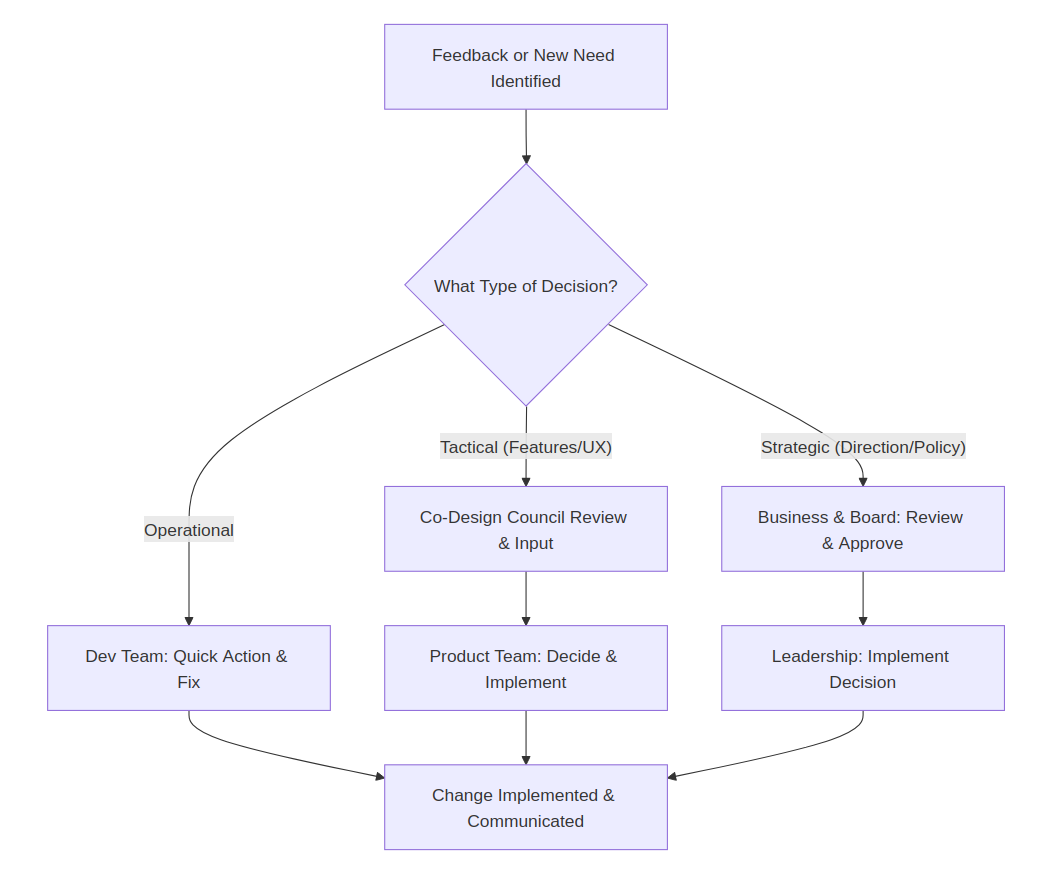
\includegraphics[keepaspectratio]{./images/diagram-shlomo.png}}

}

\caption{Diagram of the Decision-Making Process}

\end{figure}%

\section{3. Flowchart/System Architecture
Diagram}\label{flowchartsystem-architecture-diagram}

\begin{figure}[H]

{\centering \pandocbounded{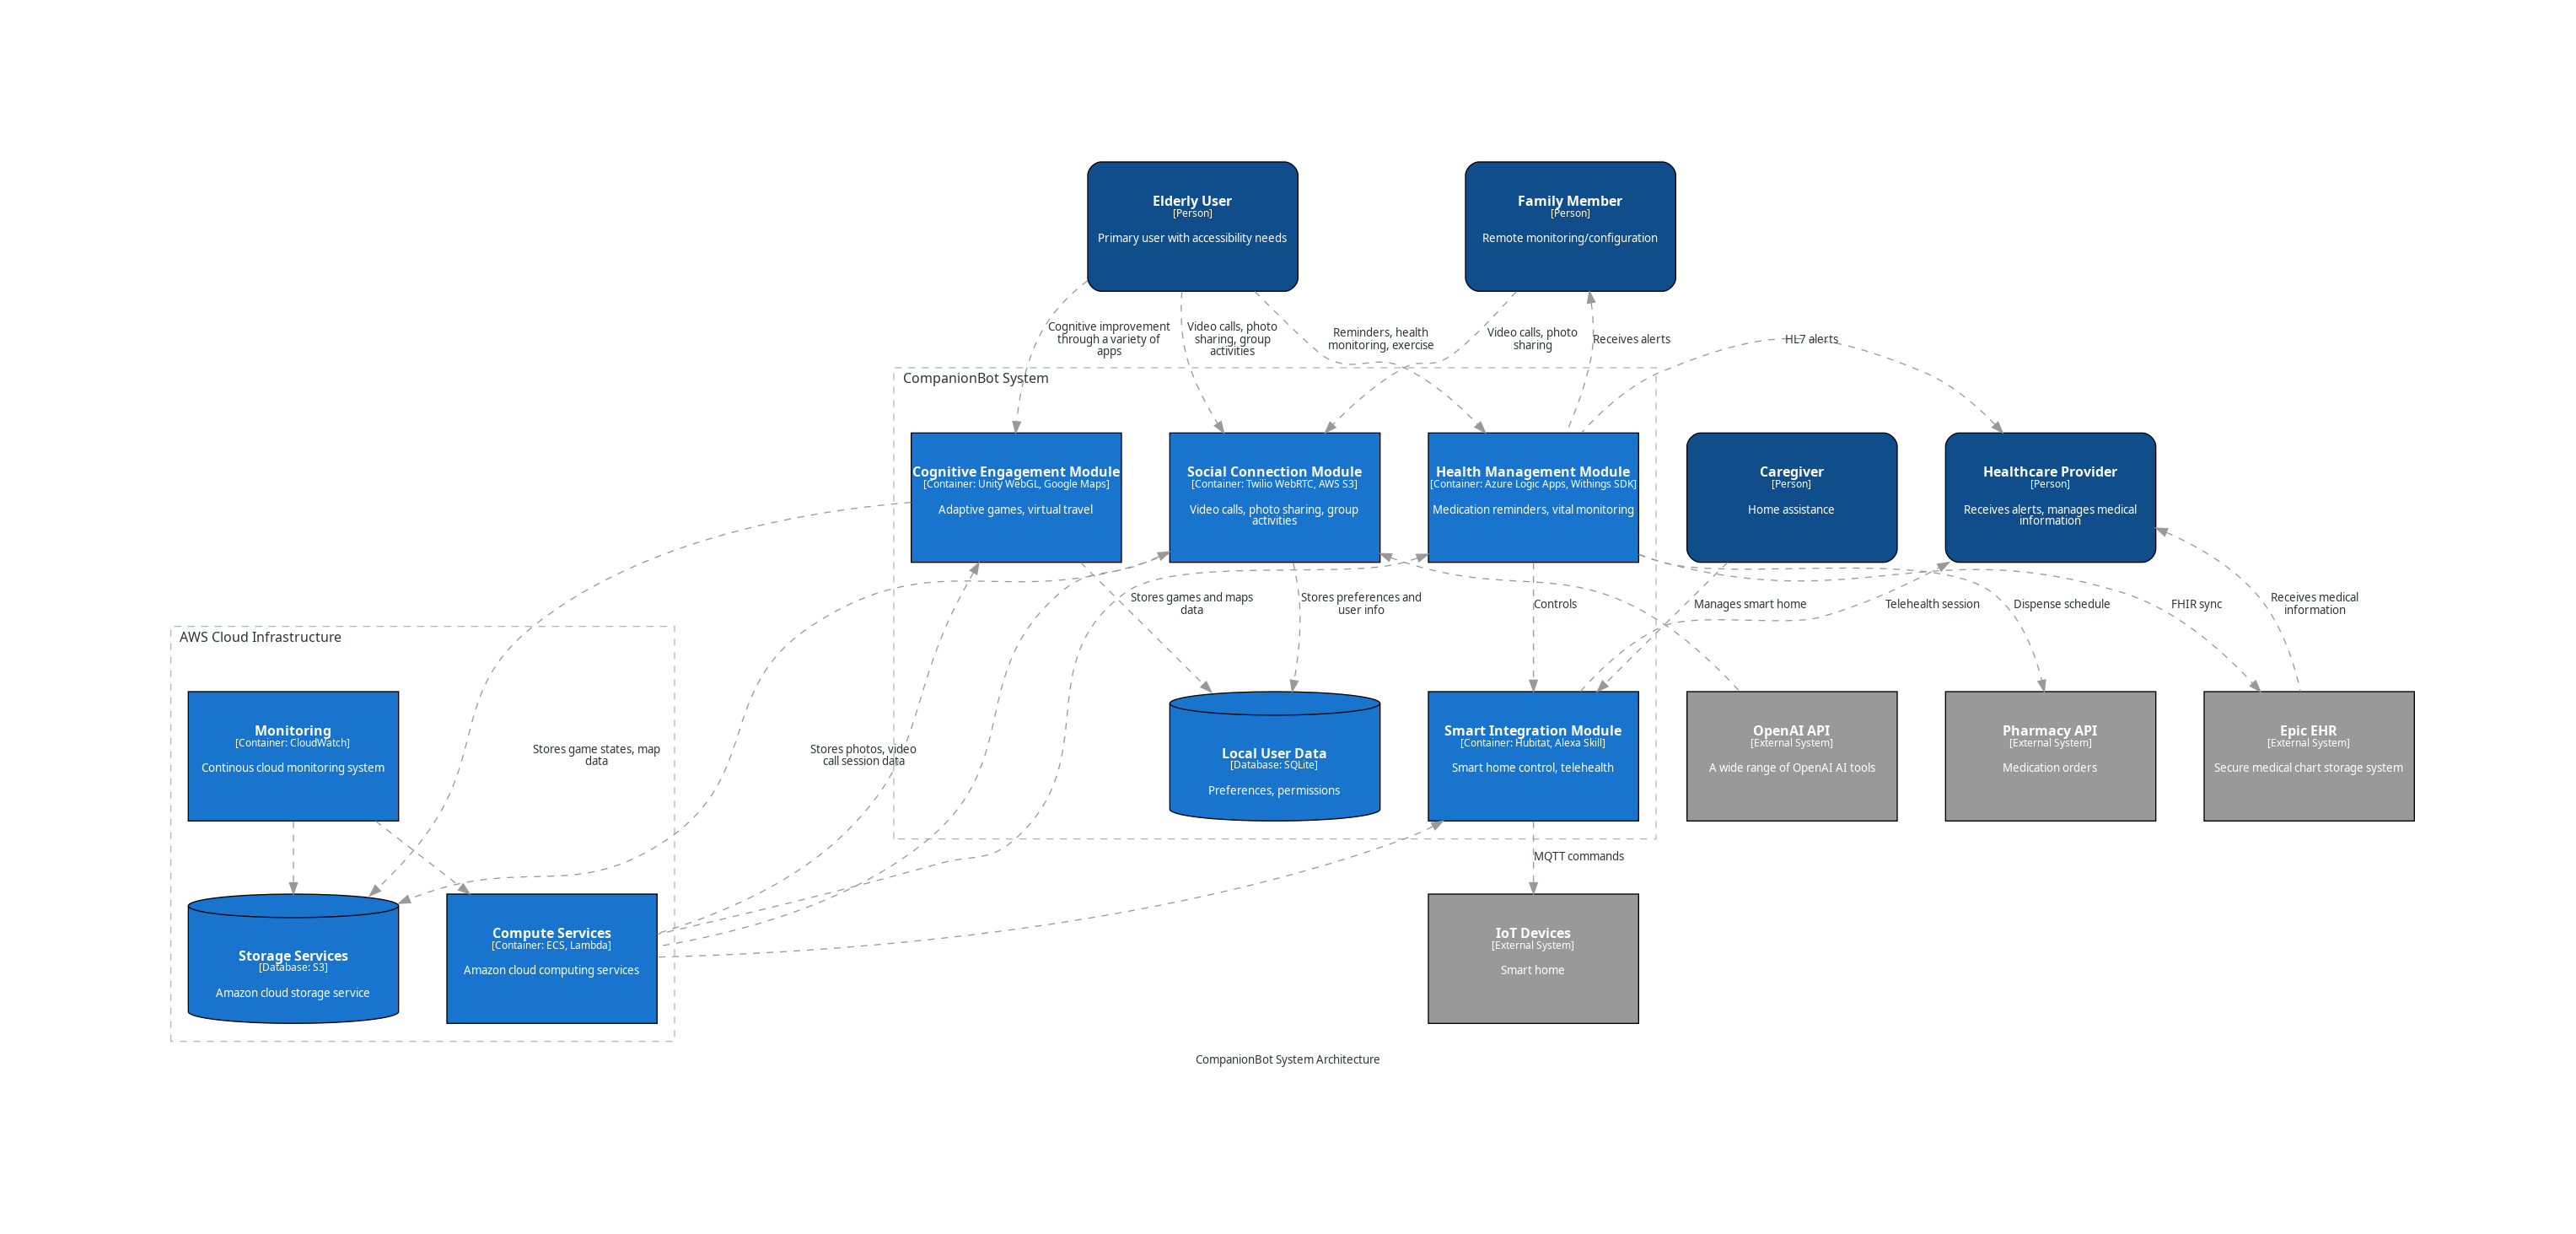
\includegraphics[keepaspectratio]{./images/companionbot_system_architecture.png}}

}

\caption{System Architecture Diagram in a C4 Standardized Format}

\end{figure}%

\section{4. Resources Required for System
Development}\label{resources-required-for-system-development}

Launching CompanionBot from prototype to full-scale deployment requires
a coordinated combination of human capital, technical tools,
infrastructure, and strategic partnerships. This chapter outlines the
essential resources---tangible and intangible---necessary for a
successful initial rollout.

\subsection{1. Human Resources}\label{human-resources}

\subsubsection{Product Team}\label{product-team}

\begin{itemize}
\tightlist
\item
  Product Owner / Product Manager -- Prioritizes features and aligns
  user needs with technical capabilities.
\item
  UX/UI Designer -- Specializes in interfaces tailored for elderly users
  and individuals with cognitive impairments.
\item
  User Researcher -- Gathers insights through interviews, usability
  testing, and interaction analytics.
\item
  Data Analyst -- Analyzes behavioral data, conducts A/B testing, and
  generates hypotheses for product improvement.
\item
  Stakeholder Liaison -- Communicates with user councils, medical
  partners, families, and social workers.
\end{itemize}

\subsubsection{Development Team}\label{development-team}

\begin{itemize}
\tightlist
\item
  AI/ML Engineers --- Implement emotion recognition, personalization,
  NLP, and adaptive learning algorithms.
\item
  Data Scientists --- Analyze real-world feedback and fine-tune AI
  behavior and decision-making logic.
\item
  Software Developers --- Skilled in Python, C, C++, Go, Rust, and
  embedded systems for backend integration and frontend interface.
\item
  Hardware Engineers --- Finalize robot shell, mobility components, and
  smart home integration features.
\item
  QA Engineers --- Test edge cases, accessibility scenarios, and
  interaction reliability.
\end{itemize}

\subsubsection{Specialized Roles}\label{specialized-roles}

\begin{itemize}
\tightlist
\item
  Gerontologists \& Geriatric Psychologists --- Guide interaction models
  and validate mental health features.
\item
  Clinical Advisors (MDs, RNs) --- Verify medical protocol compliance
  (medication reminders, vital tracking).
\item
  Speech-Language Pathologists --- Evaluate voice interface clarity and
  communication design.
\item
  Ethics and Privacy Consultants --- Ensure adherence to HIPAA, GDPR,
  and ethical AI practices.
\item
  Community Engagement Coordinators --- Onboard elderly users, provide
  training, and gather feedback.
\end{itemize}

\subsubsection{Support \& Operations}\label{support-operations}

\begin{itemize}
\tightlist
\item
  Customer Support Staff --- Trained in elder tech use and empathetic
  communication.
\item
  Sales and Partnership Managers --- Drive institutional and healthcare
  adoption.
\item
  Training Specialists --- For family members and caregivers.
\end{itemize}

\subsection{2. Technical and Digital
Infrastructure}\label{technical-and-digital-infrastructure}

\textbf{Hardware Components}

\begin{itemize}
\tightlist
\item
  Final production version of CompanionBot device with:

  \begin{itemize}
  \tightlist
  \item
    High-resolution screen and wide-angle camera
  \item
    Emotion-expressive LED facial interface
  \item
    Microphone arrays with noise cancellation
  \item
    Speakers with adjustable volume and voice clarity optimization
  \item
    Embedded sensors (touch, motion, temperature, fall detection)
  \item
    Long-life rechargeable battery with safety certification
  \item
    Smart home integration modules (Wi-Fi, Bluetooth, Zigbee, etc.)
  \item
    Telehealth peripherals integration (e.g., BP monitor, pulse
    oximeter, thermometer)
  \end{itemize}
\end{itemize}

\textbf{Software Platforms}

\begin{itemize}
\tightlist
\item
  Natural Language Processing Engine (transformer-based)
\item
  Emotion Recognition Framework (computer vision and vocal analysis)
\item
  Behavioral Analytics Engine (real-time analysis of routines, habits,
  and engagement trends)
\item
  System OS (lightweight, secure, modular, OTA updates)
\item
  User Interface (custom elderly-friendly launcher, customizable
  layouts)
\item
  Data Sync \& Cloud Services (secure AWS hosting with local fallback)
\end{itemize}

\textbf{Data \& Integration Tools}

\begin{itemize}
\tightlist
\item
  EHR/EMR Interoperability API layer (FHIR-compliant)
\item
  Caregiver dashboard (web and mobile)
\item
  Remote configuration and analytics tools for families
\item
  Voice control for accessibility
\end{itemize}

\subsection{3. Organizational and Business
Resources}\label{organizational-and-business-resources}

\begin{itemize}
\tightlist
\item
  CRM and customer support platforms
\item
  Training modules for users and caregivers (digital + in-person)
\item
  Pilot program toolkit (onboarding, usage guides, evaluation metrics)
\end{itemize}

\textbf{Marketing \& Outreach}

\begin{itemize}
\tightlist
\item
  Educational content explaining AI and robot ethics
\item
  Community events, webinars, and co-design workshops
\item
  Partnerships with elder care NGOs, clinics, and municipalities
\end{itemize}

\subsection{4. Financial Resources}\label{financial-resources}

\textbf{Initial Capital}

Seed or Series A funding to cover:

\begin{itemize}
\tightlist
\item
  Manufacturing (pilot batch)
\item
  Team salaries (12--18 months runway)
\item
  Regulatory and certification costs
\item
  Legal, insurance, and compliance auditing
\item
  Marketing and community onboarding
\item
  Infrastructure (cloud, devices, integration licenses)
\end{itemize}

\textbf{Ongoing Funding Strategy}

\begin{itemize}
\tightlist
\item
  Grants from public health and aging-focused institutions
\item
  Strategic corporate partnerships (e.g., smart home vendors, insurers)
\item
  Subscription revenue and B2B sales (senior care homes, health systems)
\end{itemize}

\subsection{5. Legal and Compliance
Resources}\label{legal-and-compliance-resources}

\begin{itemize}
\tightlist
\item
  Accessibility audit and WCAG 2.1 testing tools
\item
  Regulatory consultant team for device certifications (FDA/CE if
  applicable)
\item
  Consent management frameworks for families and healthcare providers
\end{itemize}

\subsection{6. Launch-Ready Metrics and
KPIs}\label{launch-ready-metrics-and-kpis}

To evaluate resource adequacy and deployment readiness, the following
benchmarks must be met:

\begin{itemize}
\tightlist
\item
  95\%+ success rate in daily use test scenarios with seniors
\item
  90\% of Co-Design Council UX priorities implemented
\item
  100\% of privacy and regulatory protocols certified
\item
  Functional integration with at least 3 EHR systems
\item
  Scalable cloud infrastructure deployed in 2+ regions
\item
  Fully trained customer support and caregiver enablement teams
\item
  Positive sentiment in \textgreater80\% of beta tester feedback
  sessions
\end{itemize}

\begin{quote}
A successful CompanionBot launch requires more than just technology ---
it requires a full ecosystem of specialized expertise, empathetic
design, trusted infrastructure, and inclusive partnerships. By ensuring
these resources are secured and aligned with the system's mission, we
can deliver not just a product, but a meaningful support system for the
aging population.
\end{quote}

\section{5. Detailed List of Tasks and Required
Resources}\label{detailed-list-of-tasks-and-required-resources}

Below is a structured, detailed breakdown of all specific tasks
(engineering, design, training, validation, etc.), responsible roles or
teams, and crucial resources. Tasks are organized by system components,
e.g., conversation UI, health monitoring, emotion recognition, etc.,
based on the modules and features of the system.

\begin{longtable}[]{@{}
  >{\raggedright\arraybackslash}p{(\linewidth - 12\tabcolsep) * \real{0.0620}}
  >{\raggedright\arraybackslash}p{(\linewidth - 12\tabcolsep) * \real{0.1395}}
  >{\raggedright\arraybackslash}p{(\linewidth - 12\tabcolsep) * \real{0.1628}}
  >{\raggedright\arraybackslash}p{(\linewidth - 12\tabcolsep) * \real{0.1473}}
  >{\raggedright\arraybackslash}p{(\linewidth - 12\tabcolsep) * \real{0.1395}}
  >{\raggedright\arraybackslash}p{(\linewidth - 12\tabcolsep) * \real{0.2016}}
  >{\raggedright\arraybackslash}p{(\linewidth - 12\tabcolsep) * \real{0.1473}}@{}}
\toprule\noalign{}
\begin{minipage}[b]{\linewidth}\raggedright
Task ID
\end{minipage} & \begin{minipage}[b]{\linewidth}\raggedright
Task Description
\end{minipage} & \begin{minipage}[b]{\linewidth}\raggedright
Responsible Role(s)
\end{minipage} & \begin{minipage}[b]{\linewidth}\raggedright
Required Resources
\end{minipage} & \begin{minipage}[b]{\linewidth}\raggedright
LLM Contribution
\end{minipage} & \begin{minipage}[b]{\linewidth}\raggedright
Impact on User Experience
\end{minipage} & \begin{minipage}[b]{\linewidth}\raggedright
Development Phase
\end{minipage} \\
\midrule\noalign{}
\endhead
\bottomrule\noalign{}
\endlastfoot
T1 & Define user scenarios \& elderly personas & UX Designer,
Gerontologist & Stakeholder input, Co-design council feedback & Not
directly involved in this phase, but user data helps fine-tune future
prompts and personalization logic. & Scenarios built here guide how LLM
conversations align with real user needs. & Phase 1 \\
T2 & Design conversational UI (voice interface) & UX Designer, Speech
Pathologist & GPT-based LLM, voice SDKs & Drives natural and
context-rich dialogue via fine-tuned LLM & Allows seniors to hold
meaningful daily conversations with the robot & Phase 2 \\
T3 & Develop emotion recognition module & AI/ML Engineer & GPU
infrastructure, camera, dataset for emotions & The LLM uses emotional
input (voice tone, facial expression, textual sentiment) to adapt its
language generation in real-time --- expressing empathy, changing tone,
or adjusting conversation flow. LLM also helps in labeling or
classifying emotional context during post-processing and learning loops.
& Users feel emotionally understood and cared for. The robot's ability
to respond with warmth, support, or cheer based on emotional state
builds trust and reduces feelings of loneliness. Emotional alignment is
key to senior engagement. & Phase 2 \\
T4 & Program medication reminder logic & Software Developer, MD Advisor
& Medication protocols, NLP engine & Generates adaptive and polite
reminder phrasing using prompt engineering & Improves medication
adherence through trust and tone personalization & Phase 2 \\
T5 & Implement video calling \& photo sharing features & Software
Developer, UI Designer & Camera integration, UI frameworks & Helps
narrate and format photo captions or life stories using natural language
& Assists seniors in building digital memoirs without typing or
technical complexity & Phase 3 \\
T6 & Build smart home control module & Embedded System Engineer & IoT
SDKs, Zigbee/Bluetooth modules & Converts natural spoken commands into
smart home actions via voice interface. & Users feel empowered
controlling their home by speaking casually, with no technical
knowledge. & Phase 3 \\
T7 & Design and train cognitive games & AI/ML Engineer, Cognitive
Psychologist & Puzzle DB, training datasets & Creates or adapts word
games, storytelling prompts, quizzes dynamically & Keeps engagement
fresh and tailored to cognitive ability levels & Phase 3 \\
T8 & Integrate health sensors (e.g., BP monitor) & Hardware Engineer,
RN/MD & Health devices, API integration & Explains health data to the
user in understandable language; answers health-related questions
conversationally. & Increases users' sense of control over their health;
reduces confusion or anxiety. & Phase 3 \\
T9 & Perform clinical safety validation & QA Engineer, Clinical Advisor
& Test environments, elderly beta testers & N/A & N/A & Phase 4 \\
T10 & Ensure data encryption and HIPAA compliance & Privacy Officer,
DevSecOps & Security framework & Handles sensitive discussions like data
use or family sharing in clear language & Boosts trust and comprehension
of legal/ethical concepts & Phase 4 \\
T11 & Conduct usability testing with seniors & User Researcher, Support
Staff & Demo units, testing labs & LLM interprets real-time user
feedback during sessions & Enables rapid personalization and identifies
frustration triggers & Phase 4 \\
T12 & Deploy pilot version in test homes & Ops Team, Customer Support &
10-20 pilot units, feedback tracking & Analyzes in-product textual or
verbal feedback for sentiment/emotion detection & Allows automatic
system adaptation based on user satisfaction & Phase 5 \\
T13 & Train caregivers and family on dashboard & Training Specialist &
Online modules, guides, live support & LLM acts as an assistant to
explain dashboard elements conversationally or via chatbot. & Reduces
technical barriers for family/caregivers; improves support continuity. &
Phase 5 \\
T14 & Final QA \& bug fixing pre-launch & QA Team, Dev Team & Issue
tracker, test automation suite & Used for automated log summarization or
detecting anomalies in user logs (e.g., misunderstanding patterns). &
Ensures smoother, more stable interactions with minimal breakdowns. &
Phase 6 \\
T15 & Launch CompanionBot \& onboarding campaign & Marketing, Sales,
Support & CRM, webinars, NGO partnerships & LLM supports onboarding
script personalization and FAQ chatbot for new users and families. &
Reduces onboarding stress and improves adoption rates across different
cognitive levels. & Phase 6 \\
\end{longtable}

\section{6. Evaluation of Scheduling and Prioritization of Tasks and
Resources}\label{evaluation-of-scheduling-and-prioritization-of-tasks-and-resources}

\subsection{1. Framework Overview}\label{framework-overview}

The CompanionBot project represents a complex AI-driven healthcare
technology initiative requiring sophisticated resource management and
task prioritization strategies. This evaluation examines the systematic
approach to scheduling and resource allocation that ensures optimal
project outcomes while maintaining quality standards and regulatory
compliance. The framework balances stakeholder needs, technical
constraints, and market demands through a multi-dimensional approach
that considers human capital, technical infrastructure, financial
resources, and time dependencies.

The success of CompanionBot depends not only on resource availability
but also on strategic allocation and implementation of robust
prioritization mechanisms that adapt to changing requirements and
emerging challenges in elderly care technology development.

\subsection{2. Resource Classification and Strategic
Allocation}\label{resource-classification-and-strategic-allocation}

\subsubsection{Human Resource
Distribution}\label{human-resource-distribution}

The project's human resource strategy follows a structured hierarchy
ensuring optimal skill utilization while maintaining clear
accountability. The allocation reflects the project's emphasis on
user-centered design and regulatory compliance.

\begin{longtable}[]{@{}
  >{\raggedright\arraybackslash}p{(\linewidth - 8\tabcolsep) * \real{0.2035}}
  >{\raggedright\arraybackslash}p{(\linewidth - 8\tabcolsep) * \real{0.1062}}
  >{\raggedright\arraybackslash}p{(\linewidth - 8\tabcolsep) * \real{0.1327}}
  >{\raggedright\arraybackslash}p{(\linewidth - 8\tabcolsep) * \real{0.4071}}
  >{\raggedright\arraybackslash}p{(\linewidth - 8\tabcolsep) * \real{0.1504}}@{}}
\toprule\noalign{}
\begin{minipage}[b]{\linewidth}\raggedright
Resource Category
\end{minipage} & \begin{minipage}[b]{\linewidth}\raggedright
Allocation
\end{minipage} & \begin{minipage}[b]{\linewidth}\raggedright
Priority Level
\end{minipage} & \begin{minipage}[b]{\linewidth}\raggedright
Key Roles
\end{minipage} & \begin{minipage}[b]{\linewidth}\raggedright
Timeline Focus
\end{minipage} \\
\midrule\noalign{}
\endhead
\bottomrule\noalign{}
\endlastfoot
Product Leadership & 15\% & Critical & Product Manager, UX Designer,
User Researcher & Phases 1-6 \\
Core Development & 35\% & Critical & AI/ML Engineers, Software
Developers, Hardware Engineers & Phases 2-5 \\
Specialized Expertise & 20\% & High & Data Scientists, QA Engineers,
Gerontologists & Phases 3-6 \\
Clinical Advisory & 10\% & High & MDs, RNs, Speech-Language Pathologists
& Phases 2-4 \\
Compliance \& Ethics & 8\% & Critical & Privacy Officers, Ethics
Advisors & Phases 1-6 \\
Support Operations & 12\% & Medium & Customer Support, Training
Specialists & Phases 5-6 \\
\end{longtable}

\subsubsection{Technical Infrastructure
Prioritization}\label{technical-infrastructure-prioritization}

Technical infrastructure represents a significant investment requiring
careful prioritization to ensure scalability and reliability. The
allocation follows a risk-based approach where critical components
affecting user safety and regulatory compliance receive highest
priority.

\begin{longtable}[]{@{}
  >{\raggedright\arraybackslash}p{(\linewidth - 6\tabcolsep) * \real{0.2577}}
  >{\raggedright\arraybackslash}p{(\linewidth - 6\tabcolsep) * \real{0.2268}}
  >{\raggedright\arraybackslash}p{(\linewidth - 6\tabcolsep) * \real{0.1134}}
  >{\raggedright\arraybackslash}p{(\linewidth - 6\tabcolsep) * \real{0.4021}}@{}}
\toprule\noalign{}
\begin{minipage}[b]{\linewidth}\raggedright
Infrastructure Component
\end{minipage} & \begin{minipage}[b]{\linewidth}\raggedright
Investment Range
\end{minipage} & \begin{minipage}[b]{\linewidth}\raggedright
Priority
\end{minipage} & \begin{minipage}[b]{\linewidth}\raggedright
Implementation Dependencies
\end{minipage} \\
\midrule\noalign{}
\endhead
\bottomrule\noalign{}
\endlastfoot
Hardware Development & \$2.5M -- \$4M & Critical & Industrial design,
component sourcing \\
AI/ML Platform & \$800K -- \$1.2M & Critical & Data collection, model
training \\
Security Framework & \$400K -- \$600K & Critical & Legal compliance,
data protection \\
Cloud Infrastructure & \$300K -- \$500K annually & High & Security
certification, HIPAA compliance \\
Integration APIs & \$200K -- \$400K & High & EHR partnerships, smart
home vendors \\
Testing Environment & \$150K -- \$250K & Medium & Hardware prototypes,
user testing \\
\end{longtable}

\subsection{3. Task Prioritization
Methodology}\label{task-prioritization-methodology}

\subsubsection{Multi-Criteria Decision
Framework}\label{multi-criteria-decision-framework}

The project employs a sophisticated scoring system that evaluates tasks
based on multiple dimensions, ensuring systematic and transparent
resource allocation decisions.

\begin{longtable}[]{@{}
  >{\raggedright\arraybackslash}p{(\linewidth - 6\tabcolsep) * \real{0.1930}}
  >{\raggedright\arraybackslash}p{(\linewidth - 6\tabcolsep) * \real{0.0702}}
  >{\raggedright\arraybackslash}p{(\linewidth - 6\tabcolsep) * \real{0.3947}}
  >{\raggedright\arraybackslash}p{(\linewidth - 6\tabcolsep) * \real{0.3421}}@{}}
\toprule\noalign{}
\begin{minipage}[b]{\linewidth}\raggedright
Evaluation Criteria
\end{minipage} & \begin{minipage}[b]{\linewidth}\raggedright
Weight
\end{minipage} & \begin{minipage}[b]{\linewidth}\raggedright
Description
\end{minipage} & \begin{minipage}[b]{\linewidth}\raggedright
Scoring Impact
\end{minipage} \\
\midrule\noalign{}
\endhead
\bottomrule\noalign{}
\endlastfoot
User Impact & 25\% & Direct benefit to elderly users and families &
Primary driver for feature selection \\
Technical Feasibility & 20\% & Implementation complexity and risk
assessment & Prevents over-commitment to unrealistic features \\
Regulatory Compliance & 20\% & Alignment with HIPAA, GDPR, safety
requirements & Ensures legal adherence and market access \\
Stakeholder Value & 15\% & Benefit to healthcare providers and
caregivers & Supports ecosystem adoption \\
Market Differentiation & 10\% & Competitive advantage and unique value &
Drives commercial success \\
Resource Efficiency & 10\% & Cost-effectiveness and optimization &
Maintains budget discipline \\
\end{longtable}

\subsubsection{Feature Development Priority
Tiers}\label{feature-development-priority-tiers}

\begin{longtable}[]{@{}
  >{\raggedright\arraybackslash}p{(\linewidth - 6\tabcolsep) * \real{0.1148}}
  >{\raggedright\arraybackslash}p{(\linewidth - 6\tabcolsep) * \real{0.4098}}
  >{\raggedright\arraybackslash}p{(\linewidth - 6\tabcolsep) * \real{0.1639}}
  >{\raggedright\arraybackslash}p{(\linewidth - 6\tabcolsep) * \real{0.3115}}@{}}
\toprule\noalign{}
\begin{minipage}[b]{\linewidth}\raggedright
Priority Tier
\end{minipage} & \begin{minipage}[b]{\linewidth}\raggedright
Features
\end{minipage} & \begin{minipage}[b]{\linewidth}\raggedright
Resource Allocation
\end{minipage} & \begin{minipage}[b]{\linewidth}\raggedright
Justification
\end{minipage} \\
\midrule\noalign{}
\endhead
\bottomrule\noalign{}
\endlastfoot
Tier 1 (Critical) & Basic conversation, medication reminders, emergency
alerts & 40\% & Core safety and companionship functions \\
Tier 2 (High) & Health monitoring, family communication, cognitive games
& 35\% & Enhanced value proposition \\
Tier 3 (Medium) & Smart home integration, advanced AI personalization &
20\% & Competitive differentiation \\
Tier 4 (Low) & Advanced entertainment, complex social features & 5\% &
Future enhancement opportunities \\
\end{longtable}

\subsection{4. Development Timeline and Critical Path
Management}\label{development-timeline-and-critical-path-management}

\subsubsection{Phase-Based Development
Schedule}\label{phase-based-development-schedule}

The development follows a structured timeline that aligns resource
allocation with project milestones and stakeholder deliverables,
providing flexibility for iterative development while maintaining
accountability.

\begin{longtable}[]{@{}
  >{\raggedright\arraybackslash}p{(\linewidth - 8\tabcolsep) * \real{0.1752}}
  >{\raggedright\arraybackslash}p{(\linewidth - 8\tabcolsep) * \real{0.0803}}
  >{\raggedright\arraybackslash}p{(\linewidth - 8\tabcolsep) * \real{0.2993}}
  >{\raggedright\arraybackslash}p{(\linewidth - 8\tabcolsep) * \real{0.1679}}
  >{\raggedright\arraybackslash}p{(\linewidth - 8\tabcolsep) * \real{0.2774}}@{}}
\toprule\noalign{}
\begin{minipage}[b]{\linewidth}\raggedright
Phase
\end{minipage} & \begin{minipage}[b]{\linewidth}\raggedright
Duration
\end{minipage} & \begin{minipage}[b]{\linewidth}\raggedright
Key Deliverables
\end{minipage} & \begin{minipage}[b]{\linewidth}\raggedright
Resource Focus
\end{minipage} & \begin{minipage}[b]{\linewidth}\raggedright
Success Metrics
\end{minipage} \\
\midrule\noalign{}
\endhead
\bottomrule\noalign{}
\endlastfoot
Phase 1: Foundation & 3 months & Requirements, architecture, team
assembly & Product team, infrastructure & Stakeholder approval,
technical feasibility \\
Phase 2: Core Development & 6 months & Basic AI, hardware prototype,
safety features & Development team, clinical advisors & Functional
prototype, safety validation \\
Phase 3: Integration & 4 months & System integration, initial testing &
Full team, testing infrastructure & Integration testing, user
acceptance \\
Phase 4: Validation & 3 months & Clinical trials, regulatory approval &
Compliance team, clinical partners & Regulatory clearance, user
validation \\
Phase 5: Pilot Deployment & 2 months & Limited release, user training &
Support team, training specialists & User adoption, feedback
collection \\
Phase 6: Full Launch & 2 months & Market launch, scaling operations &
Marketing, operations team & Market penetration, operational
efficiency \\
\end{longtable}

\subsubsection{Critical Path Analysis}\label{critical-path-analysis}

\begin{longtable}[]{@{}
  >{\raggedright\arraybackslash}p{(\linewidth - 8\tabcolsep) * \real{0.1544}}
  >{\raggedright\arraybackslash}p{(\linewidth - 8\tabcolsep) * \real{0.0738}}
  >{\raggedright\arraybackslash}p{(\linewidth - 8\tabcolsep) * \real{0.2752}}
  >{\raggedright\arraybackslash}p{(\linewidth - 8\tabcolsep) * \real{0.2483}}
  >{\raggedright\arraybackslash}p{(\linewidth - 8\tabcolsep) * \real{0.2483}}@{}}
\toprule\noalign{}
\begin{minipage}[b]{\linewidth}\raggedright
Critical Activity
\end{minipage} & \begin{minipage}[b]{\linewidth}\raggedright
Duration
\end{minipage} & \begin{minipage}[b]{\linewidth}\raggedright
Resource Requirements
\end{minipage} & \begin{minipage}[b]{\linewidth}\raggedright
Risk Factors
\end{minipage} & \begin{minipage}[b]{\linewidth}\raggedright
Mitigation Strategy
\end{minipage} \\
\midrule\noalign{}
\endhead
\bottomrule\noalign{}
\endlastfoot
AI Model Development & 4 months & 3 AI engineers, compute resources &
Model performance, training data quality & Parallel algorithm
development, data augmentation \\
Hardware Certification & 3 months & Hardware team, testing lab &
Regulatory approval, component availability & Early prototype testing,
supplier diversification \\
Clinical Validation & 2 months & Clinical advisors, test sites & User
acceptance, health outcome validation & Phased testing approach,
multiple validation sites \\
Security Audit & 1.5 months & Security team, external auditors &
Vulnerability discovery, compliance gaps & Continuous security testing,
expert consultation \\
\end{longtable}

\subsection{5. Performance Monitoring and
Optimization}\label{performance-monitoring-and-optimization}

\subsubsection{Resource Utilization
Metrics}\label{resource-utilization-metrics}

Effective resource management requires continuous monitoring of
utilization rates and efficiency metrics to identify optimization
opportunities and ensure project objectives are met within constraints.

\begin{longtable}[]{@{}
  >{\raggedright\arraybackslash}p{(\linewidth - 8\tabcolsep) * \real{0.1756}}
  >{\raggedright\arraybackslash}p{(\linewidth - 8\tabcolsep) * \real{0.2061}}
  >{\raggedright\arraybackslash}p{(\linewidth - 8\tabcolsep) * \real{0.1603}}
  >{\raggedright\arraybackslash}p{(\linewidth - 8\tabcolsep) * \real{0.1603}}
  >{\raggedright\arraybackslash}p{(\linewidth - 8\tabcolsep) * \real{0.2977}}@{}}
\toprule\noalign{}
\begin{minipage}[b]{\linewidth}\raggedright
Metric Category
\end{minipage} & \begin{minipage}[b]{\linewidth}\raggedright
Specific Metrics
\end{minipage} & \begin{minipage}[b]{\linewidth}\raggedright
Target Range
\end{minipage} & \begin{minipage}[b]{\linewidth}\raggedright
Monitoring Frequency
\end{minipage} & \begin{minipage}[b]{\linewidth}\raggedright
Corrective Actions
\end{minipage} \\
\midrule\noalign{}
\endhead
\bottomrule\noalign{}
\endlastfoot
Budget Utilization & Spend rate, variance from plan & ±5\% of planned &
Weekly & Budget reallocation, scope adjustment \\
Timeline Adherence & Milestone completion, critical path delays & 95\%
on-time & Daily & Resource reallocation, parallel activities \\
Team Productivity & Story points completed, velocity trends & 85-110\%
of baseline & Sprint cycles & Team optimization, skill development \\
Quality Metrics & Defect rates, user acceptance scores & \textless2\%
defects, \textgreater90\% acceptance & Continuous & Quality process
improvement \\
Stakeholder Satisfaction & Feedback scores, engagement levels &
\textgreater80\% satisfaction & Monthly & Communication improvement,
expectation management \\
\end{longtable}

\textbf{Dynamic Resource Allocation Strategy}

\begin{longtable}[]{@{}
  >{\raggedright\arraybackslash}p{(\linewidth - 6\tabcolsep) * \real{0.2018}}
  >{\raggedright\arraybackslash}p{(\linewidth - 6\tabcolsep) * \real{0.2477}}
  >{\raggedright\arraybackslash}p{(\linewidth - 6\tabcolsep) * \real{0.1927}}
  >{\raggedright\arraybackslash}p{(\linewidth - 6\tabcolsep) * \real{0.3578}}@{}}
\toprule\noalign{}
\begin{minipage}[b]{\linewidth}\raggedright
Trigger Event
\end{minipage} & \begin{minipage}[b]{\linewidth}\raggedright
Response Strategy
\end{minipage} & \begin{minipage}[b]{\linewidth}\raggedright
Resource Impact
\end{minipage} & \begin{minipage}[b]{\linewidth}\raggedright
Timeline Adjustment
\end{minipage} \\
\midrule\noalign{}
\endhead
\bottomrule\noalign{}
\endlastfoot
Technical Breakthrough & Accelerate related development & +20\% to
breakthrough area & Potential timeline compression \\
Regulatory Delay & Shift focus to parallel activities & Reallocate
compliance resources & Maintain overall timeline \\
User Feedback & Prioritize user-requested features & Adjust feature
development allocation & Minor timeline impact \\
Competitive Pressure & Accelerate differentiation features & +15\% to
competitive features & Potential scope adjustment \\
\end{longtable}

\subsection{6. Financial Resource Management and Risk
Mitigation}\label{financial-resource-management-and-risk-mitigation}

\subsubsection{Budget Allocation and
Optimization}\label{budget-allocation-and-optimization}

The financial framework balances immediate development needs with
long-term sustainability requirements while maintaining adequate
reserves for risk management.

\begin{longtable}[]{@{}
  >{\raggedright\arraybackslash}p{(\linewidth - 8\tabcolsep) * \real{0.1679}}
  >{\raggedright\arraybackslash}p{(\linewidth - 8\tabcolsep) * \real{0.0916}}
  >{\raggedright\arraybackslash}p{(\linewidth - 8\tabcolsep) * \real{0.1603}}
  >{\raggedright\arraybackslash}p{(\linewidth - 8\tabcolsep) * \real{0.2901}}
  >{\raggedright\arraybackslash}p{(\linewidth - 8\tabcolsep) * \real{0.2901}}@{}}
\toprule\noalign{}
\begin{minipage}[b]{\linewidth}\raggedright
Budget Category
\end{minipage} & \begin{minipage}[b]{\linewidth}\raggedright
Percentage
\end{minipage} & \begin{minipage}[b]{\linewidth}\raggedright
Amount Range
\end{minipage} & \begin{minipage}[b]{\linewidth}\raggedright
Justification
\end{minipage} & \begin{minipage}[b]{\linewidth}\raggedright
Optimization Strategy
\end{minipage} \\
\midrule\noalign{}
\endhead
\bottomrule\noalign{}
\endlastfoot
Personnel Costs & 60\% & \$3.6M -- \$6M & Core team expertise,
specialized skills & Agile development, skill sharing \\
Technology Infrastructure & 20\% & \$1.2M -- \$2M & Hardware, software,
cloud services & Open source integration, partnerships \\
Compliance \& Legal & 8\% & \$480K -- \$800K & Regulatory requirements,
IP protection & Early compliance planning, automation \\
Marketing \& Sales & 7\% & \$420K -- \$700K & Market entry, customer
acquisition & Digital marketing, strategic partnerships \\
Operations \& Support & 3\% & \$180K -- \$300K & Customer service,
maintenance & Self-service tools, automation \\
Contingency & 2\% & \$120K -- \$200K & Risk mitigation, unexpected costs
& Risk-based allocation, flexible reserves \\
\end{longtable}

\subsection{7. Quality Assurance and Compliance Resource
Allocation}\label{quality-assurance-and-compliance-resource-allocation}

\subsubsection{Quality-Driven Resource
Distribution}\label{quality-driven-resource-distribution}

Quality assurance requires dedicated allocation across all development
phases to ensure safety, usability, and reliability standards for
elderly care applications.

\begin{longtable}[]{@{}
  >{\raggedright\arraybackslash}p{(\linewidth - 6\tabcolsep) * \real{0.1760}}
  >{\raggedright\arraybackslash}p{(\linewidth - 6\tabcolsep) * \real{0.2160}}
  >{\raggedright\arraybackslash}p{(\linewidth - 6\tabcolsep) * \real{0.3040}}
  >{\raggedright\arraybackslash}p{(\linewidth - 6\tabcolsep) * \real{0.3040}}@{}}
\toprule\noalign{}
\begin{minipage}[b]{\linewidth}\raggedright
QA Activity
\end{minipage} & \begin{minipage}[b]{\linewidth}\raggedright
Resource Allocation
\end{minipage} & \begin{minipage}[b]{\linewidth}\raggedright
Quality Metrics
\end{minipage} & \begin{minipage}[b]{\linewidth}\raggedright
Success Criteria
\end{minipage} \\
\midrule\noalign{}
\endhead
\bottomrule\noalign{}
\endlastfoot
Requirements Validation & 10\% of QA budget & Requirements coverage,
stakeholder approval & 100\% requirement validation \\
Design Review & 15\% of QA budget & Design compliance, usability scores
& 95\% design approval rate \\
Code Quality & 25\% of QA budget & Code coverage, defect density &
\textless2 defects per KLOC \\
Integration Testing & 20\% of QA budget & System integration success &
98\% integration test pass rate \\
User Acceptance & 20\% of QA budget & User satisfaction, usability
metrics & 90\% user acceptance rate \\
Compliance Validation & 10\% of QA budget & Regulatory compliance,
security audit & 100\% compliance certification \\
\end{longtable}

\subsubsection{Risk-Based Testing
Strategy}\label{risk-based-testing-strategy}

Testing strategy prioritizes high-risk areas that could impact user
safety or system reliability, ensuring critical functionality receives
appropriate resources.

\begin{longtable}[]{@{}
  >{\raggedright\arraybackslash}p{(\linewidth - 6\tabcolsep) * \real{0.2245}}
  >{\raggedright\arraybackslash}p{(\linewidth - 6\tabcolsep) * \real{0.1224}}
  >{\raggedright\arraybackslash}p{(\linewidth - 6\tabcolsep) * \real{0.2653}}
  >{\raggedright\arraybackslash}p{(\linewidth - 6\tabcolsep) * \real{0.3878}}@{}}
\toprule\noalign{}
\begin{minipage}[b]{\linewidth}\raggedright
Risk Area
\end{minipage} & \begin{minipage}[b]{\linewidth}\raggedright
Risk Level
\end{minipage} & \begin{minipage}[b]{\linewidth}\raggedright
Testing Resources
\end{minipage} & \begin{minipage}[b]{\linewidth}\raggedright
Acceptance Criteria
\end{minipage} \\
\midrule\noalign{}
\endhead
\bottomrule\noalign{}
\endlastfoot
Medication Reminders & Critical & 30\% of testing budget & 99.9\%
reliability \\
Emergency Alerts & Critical & 25\% of testing budget & 100\% alert
delivery \\
Health Data Security & Critical & 20\% of testing budget & Zero security
vulnerabilities \\
User Interface & High & 15\% of testing budget & 95\% usability score \\
AI Interactions & High & 10\% of testing budget & 90\% appropriate
response rate \\
\end{longtable}

\section{7. Dependency Identification}\label{dependency-identification}

The successful implementation of CompanionBot relies on the coordinated
interaction of multiple technical systems, organizational roles,
external vendors, and regulatory frameworks. Identifying and managing
these dependencies early is essential to ensure uninterrupted
development, maintain system integrity, and support compliance with
safety and privacy standards.

\subsection{Technical Dependencies}\label{technical-dependencies}

\begin{itemize}
\tightlist
\item
  \textbf{Large Language Model (LLM) API:} All conversational,
  emotional, and adaptive personalization features are dependent on the
  performance and availability of the LLM engine.
\item
  \textbf{Health Monitoring Sensors:} Integration with medical
  peripherals (e.g., blood pressure monitors, oximeters) is dependent on
  device-specific APIs and reliable Bluetooth/Zigbee communication
  protocols.
\item
  \textbf{AWS Cloud Synchronization:} System behavior depends on stable
  cloud connectivity for data persistence, analytics, and user profile
  management, with fallback mechanisms for offline usage.
\item
  \textbf{Telehealth and EHR Integration:} Interoperability with
  external health systems (FHIR APIs) requires alignment with
  third-party update cycles and interface changes.
\end{itemize}

\subsection{Organizational and Process
Dependencies}\label{organizational-and-process-dependencies}

\begin{itemize}
\tightlist
\item
  \textbf{Stakeholder Feedback Loops:} The Co-Design Council and
  caregiver testing groups play a central role in interface and feature
  prioritization. Development sprints depend on timely input and
  validation cycles.
\item
  \textbf{Cross-Team Coordination:} Seamless delivery requires
  synchronization between AI/ML, UX, clinical advisors, and various
  consultants. Bottlenecks in one team may delay dependent components.
\item
  \textbf{Training Resources for Families and Caregivers:} Deployment
  success depends on the creation and dissemination of training modules,
  which are reliant on the availability of support staff and content
  specialists.
\end{itemize}

\subsection{Vendor and Regulatory
Dependencies}\label{vendor-and-regulatory-dependencies}

\begin{itemize}
\tightlist
\item
  \textbf{Hardware Supply Chain:} All hardware components are sourced
  externally. Delays in component delivery can affect assembly and
  testing milestones.
\item
  \textbf{Compliance Certifications:} Deployment hinges on timely
  security audits and HIPAA/SOC2 validations, which require coordination
  with external compliance experts and auditors.
\item
  \textbf{Partnerships with Elder-Care Facilities, Clinics, and NGOs:}
  Access to pilot environments and user feedback is contingent on
  third-party collaboration timelines, legal agreements, and
  site-specific onboarding procedures.
\end{itemize}

\subsection{Mitigation Strategies}\label{mitigation-strategies}

\begin{itemize}
\tightlist
\item
  \textbf{Live Dependency Register:} Maintained by the Project Manager
  and updated at each sprint planning session; tracks technical, legal,
  and logistical dependencies by module and development phase.
\item
  \textbf{Fallback Planning:} Local-only operation modes are implemented
  for critical features like medication reminders and emergency alerts
  in case of cloud failure or API disruption.
\item
  \textbf{Parallel Workstreams:} Tasks are decoupled where possible to
  allow non-blocking progress, e.g., UX testing on synthetic data while
  waiting for clinical validation.
\item
  \textbf{Automated Monitoring:} Integration of build systems and
  testing pipelines with dependency scanning tools ensures early
  detection of version conflicts or broken integrations.
\end{itemize}

By proactively identifying and addressing interdependencies,
CompanionBot ensures stable progress across all development phases,
while maintaining flexibility to adapt to external or internal changes.

\section{8. Identification and Assessment of Risks (in Terms of
Resources)}\label{identification-and-assessment-of-risks-in-terms-of-resources}

Effective resource management for CompanionBot requires not only
accurate allocation but also early detection of risks that may
jeopardize delivery, compliance, or system stability. This section
outlines key risk domains associated with human, technical, financial,
and regulatory resources, alongside assessment metrics and mitigation
strategies.

\subsection{Human Resource Risks}\label{human-resource-risks}

\begin{itemize}
\tightlist
\item
  \textbf{Skill Gaps in Specialized Roles:} Limited availability of
  AI/ML engineers, gerontologists, and compliance officers with relevant
  expertise may delay module implementation (e.g., emotion recognition,
  HIPAA alignment).

  \begin{itemize}
  \tightlist
  \item
    \emph{Likelihood:} High
  \item
    \emph{Impact:} Critical for core functionality
  \item
    \emph{Mitigation:} Maintain expert advisory pool, invest in parallel
    onboarding, cross-train team members.
  \end{itemize}
\item
  \textbf{Resource Turnover During Development:} Unexpected departure of
  key team members (e.g., Product Owner, UX Lead) could disrupt project
  continuity and stakeholder alignment.

  \begin{itemize}
  \tightlist
  \item
    \emph{Likelihood:} Medium
  \item
    \emph{Impact:} High on coordination and velocity
  \item
    \emph{Mitigation:} Maintain updated documentation, implement
    succession plans, ensure knowledge redundancy.
  \end{itemize}
\end{itemize}

\subsection{Technical Resource Risks}\label{technical-resource-risks}

\begin{itemize}
\tightlist
\item
  \textbf{GPU Infrastructure Limitations:} High computational demand for
  LLM inference and training could exceed available GPU resources,
  affecting emotion-aware responses and adaptive personalization.

  \begin{itemize}
  \tightlist
  \item
    \emph{Likelihood:} Medium
  \item
    \emph{Impact:} High on AI performance
  \item
    \emph{Mitigation:} Use scalable cloud compute, prioritize model
    optimization, secure compute credits from providers.
  \end{itemize}
\item
  \textbf{Hardware Supply Delays:} Delays in delivery of essential
  components (e.g., LED facial modules, embedded sensors) could stall
  prototyping and testing phases.

  \begin{itemize}
  \tightlist
  \item
    \emph{Likelihood:} High
  \item
    \emph{Impact:} Medium to high
  \item
    \emph{Mitigation:} Identify backup suppliers, pre-order critical
    parts, use modular hardware design.
  \end{itemize}
\end{itemize}

\subsection{Financial Resource Risks}\label{financial-resource-risks}

\begin{itemize}
\tightlist
\item
  \textbf{Budget Overrun Due to Compliance and Validation Costs:} Costs
  associated with legal certification, audits, and regulatory
  documentation may exceed initial estimates.

  \begin{itemize}
  \tightlist
  \item
    \emph{Likelihood:} Medium
  \item
    \emph{Impact:} High on launch schedule
  \item
    \emph{Mitigation:} Reserve contingency budget (5--10\%), engage
    compliance experts early, pursue co-funding opportunities (grants,
    institutional partners).
  \end{itemize}
\item
  \textbf{Inadequate Funding for Support and Training:} Underfunding
  post-deployment training for caregivers and families may reduce
  adoption and increase dropout rates.

  \begin{itemize}
  \tightlist
  \item
    \emph{Likelihood:} Medium
  \item
    \emph{Impact:} High on user satisfaction and system continuity
  \item
    \emph{Mitigation:} Allocate specific budget to onboarding, integrate
    LLM-powered training assistants, monitor training outcomes.
  \end{itemize}
\end{itemize}

\subsection{Regulatory and Partnership
Risks}\label{regulatory-and-partnership-risks}

\begin{itemize}
\tightlist
\item
  \textbf{Delay in Certification or Audit Outcomes:}
  Slower-than-expected regulatory feedback (e.g., HIPAA, CE) could delay
  launch or limit scope of deployment.

  \begin{itemize}
  \tightlist
  \item
    \emph{Likelihood:} Medium
  \item
    \emph{Impact:} High on go-to-market readiness
  \item
    \emph{Mitigation:} Begin audit preparation in parallel with
    development, prioritize documentation, establish direct
    communication channels with auditors.
  \end{itemize}
\item
  \textbf{Stakeholder Partnership Withdrawal:} Key pilot partners (e.g.,
  care homes or NGOs) may withdraw due to internal priorities or
  strategic changes.

  \begin{itemize}
  \tightlist
  \item
    \emph{Likelihood:} Low to medium
  \item
    \emph{Impact:} Medium on pilot phase
  \item
    \emph{Mitigation:} Diversify pilot sites, maintain regular
    engagement with partners, sign flexible MoUs.
  \end{itemize}
\end{itemize}

\subsection{Risk Monitoring and
Reporting}\label{risk-monitoring-and-reporting}

CompanionBot applies a continuous risk-tracking model:

\begin{itemize}
\tightlist
\item
  \textbf{Risk Register:} Maintained by the project management team,
  updated biweekly.
\item
  \textbf{Risk Heat Maps:} Used to visualize severity vs.~likelihood
  across categories.
\item
  \textbf{LLM-Based Analysis:} Applied to project communications and
  logs to detect signals of emerging risks (e.g., unmet deadlines,
  reduced output velocity).
\item
  \textbf{Monthly Risk Review Meetings:} Representatives from product,
  compliance, AI, and stakeholder teams realign mitigation actions.
\end{itemize}

By embedding risk identification into all resource management
activities, the CompanionBot team ensures stable progress under
realistic constraints and supports a proactive rather than reactive
delivery model.




\end{document}
